\documentclass[9pt,twocolumn,twoside,]{pnas-new}

% Use the lineno option to display guide line numbers if required.
% Note that the use of elements such as single-column equations
% may affect the guide line number alignment.


\usepackage[T1]{fontenc}
\usepackage[utf8]{inputenc}

% tightlist command for lists without linebreak
\providecommand{\tightlist}{%
  \setlength{\itemsep}{0pt}\setlength{\parskip}{0pt}}


% Pandoc citation processing
\newlength{\cslhangindent}
\setlength{\cslhangindent}{1.5em}
\newlength{\csllabelwidth}
\setlength{\csllabelwidth}{3em}
\newlength{\cslentryspacingunit} % times entry-spacing
\setlength{\cslentryspacingunit}{\parskip}
% for Pandoc 2.8 to 2.10.1
\newenvironment{cslreferences}%
  {}%
  {\par}
% For Pandoc 2.11+
\newenvironment{CSLReferences}[2] % #1 hanging-ident, #2 entry spacing
 {% don't indent paragraphs
  \setlength{\parindent}{0pt}
  % turn on hanging indent if param 1 is 1
  \ifodd #1
  \let\oldpar\par
  \def\par{\hangindent=\cslhangindent\oldpar}
  \fi
  % set entry spacing
  \setlength{\parskip}{#2\cslentryspacingunit}
 }%
 {}
\usepackage{calc}
\newcommand{\CSLBlock}[1]{#1\hfill\break}
\newcommand{\CSLLeftMargin}[1]{\parbox[t]{\csllabelwidth}{#1}}
\newcommand{\CSLRightInline}[1]{\parbox[t]{\linewidth - \csllabelwidth}{#1}\break}
\newcommand{\CSLIndent}[1]{\hspace{\cslhangindent}#1}


\templatetype{pnasresearcharticle}  % Choose template

\title{Réseau de collaborations des étudiants du cours BIO500 donné à
l'Université de Sherbrooke à l'hiver 2022}

\author[a]{Alexandre Martineau}
\author[a]{Clara Prévosto}
\author[a]{Élisabeth Roy}
\author[a]{Laura Béland}
\author[a]{Laurence Boum}

  \affil[a]{Université de Sherbrooke, Départment de biologie, 2500
Boulevard de l'Université, Sherbrooke, Québec, J1K 2R1}


% Please give the surname of the lead author for the running footer
\leadauthor{}

% Please add here a significance statement to explain the relevance of your work
\significancestatement{}


\authorcontributions{}



\correspondingauthor{\textsuperscript{} }

% Keywords are not mandatory, but authors are strongly encouraged to provide them. If provided, please include two to five keywords, separated by the pipe symbol, e.g:
 \keywords{  Bacon
number |  Centralité |  Collaboration |  Liens |  Petits mondes  } 

\begin{abstract}
Dans cet article, le réseau de collaboration des étudiants du cours
BIO500 à l'hiver 2022 de l'Université de Sherbrooke fut comparé au
réseau de type petit monde pour voir si les caractéristique d'un réseau
de collaboration peut être considéré comme un réseau de petit monde.
L'utilisation de données recueilli sur 193 étudiants concernant leur
lien les uns par rapport aux autres ont servis à faire un réseaux de
collaborations. Les analyses effectuées sur ce réseau furent l'analyse
de la corrélation entre la centralité et le nombre de lien des étudiant
et le calcul du `Bacon number'd'un des étudiants pris au hazard. Ces
analyses ont montré une corrélation non significative de la centralité
et du nombre de liens et un 'Bacon number' se situant entre 2 et 4.
Cependant, les réseaux de type petit monde devrait avoir une corrélation
entre leur centralité et leur nombre de liens et un `Bacon number' de 6
et moins. Donc ce réseau de collaboration n'a pas toutes les
caractéristiques étudiées dans cette article correspondant aux
carractéristiques des réseaux de type petit monde.
\end{abstract}

\dates{This manuscript was compiled on \today}
\doi{\url{www.pnas.org/cgi/doi/10.1073/pnas.XXXXXXXXXX}}

\begin{document}

% Optional adjustment to line up main text (after abstract) of first page with line numbers, when using both lineno and twocolumn options.
% You should only change this length when you've finalised the article contents.
\verticaladjustment{-2pt}



\maketitle
\thispagestyle{firststyle}
\ifthenelse{\boolean{shortarticle}}{\ifthenelse{\boolean{singlecolumn}}{\abscontentformatted}{\abscontent}}{}

% If your first paragraph (i.e. with the \dropcap) contains a list environment (quote, quotation, theorem, definition, enumerate, itemize...), the line after the list may have some extra indentation. If this is the case, add \parshape=0 to the end of the list environment.

\acknow{}

\hypertarget{introduction}{%
\section{Introduction}\label{introduction}}

Dans plusieurs études écologiques, les différents organismes d'un
environnement donné sont tous liés entre eux par différents lien qui les
unis. Ces liens correspondent à leur réseau de connection et permettent
de voir l'impact qu'une espèce aurait sur le reste de la population
présente. Dans ce rapport, nous nous penchons sur un type de réseau
nommé le réseau de petit monde pour savoir si les caractéristiques de ce
réseau concordent avec celles du réseau de collaborations que nous avons
obtenu. Ce dernier a été produit à partir d'une base de données des
collaborations des étudiants du cours BIO500 donné à l'Université de
Sherbrooke à l'hiver 2022. Afin de répondre à notre objectif, nous
cherchons plus précisement à savoir s'il existe une corrélation entre le
nombre de liens des étudiants entre eux et leur centralité dans leur
réseau de liens. Nous effectuons également le calcul du Bacon number
d'une des étudiante pour calculer la distance entre cette étudiante et
ses collègues du cours BIO500.

\hypertarget{muxe9thode}{%
\section{Méthode}\label{muxe9thode}}

Nous avons tout d'abord récolté les données des 193 étudiant(e)s
relié(e)s au cours BIO500, soit des étudiant(e)s inscrit(e)s au cours et
ayant collaboré avec des étudiant(e)s inscrit(e)s au cours. Nous avons
classé ces données en trois tables, l'une concernant les étudiant(e)s
avec des informations telles que l'année de début de leurs études et le
nom de leur programme d'études, la deuxième concernant les cours avec
des informations telles que le sigle du cours et le nombre de crédits du
cours et la dernière concernant les collaborations entre les
étudiant(e)s avec les informations telles que le nom des deux
étudiant(e)s et le sigle du cours dans lequel ils/elles ont collaboré.
Nous avons utilisé le logiciel R version 4.1.3 pour faire la lecture, le
nettoyage, l'injection des données et l'analyse des différentes données.
À l'aide de ces données, nous avons généré trois figures nous permettant
de répondre à notre objectif, à savoir si notre réseau se compare à un
réseau de petit monde. Pour faciliter le lien entre les données,
l'analyse et les figures, nous avons créé un script target. Nous avons
également utilisé GitHub pour faciliter le partage et le stockage des
données.

\hypertarget{ruxe9sultats}{%
\section{Résultats}\label{ruxe9sultats}}

\begin{figure}
\centering
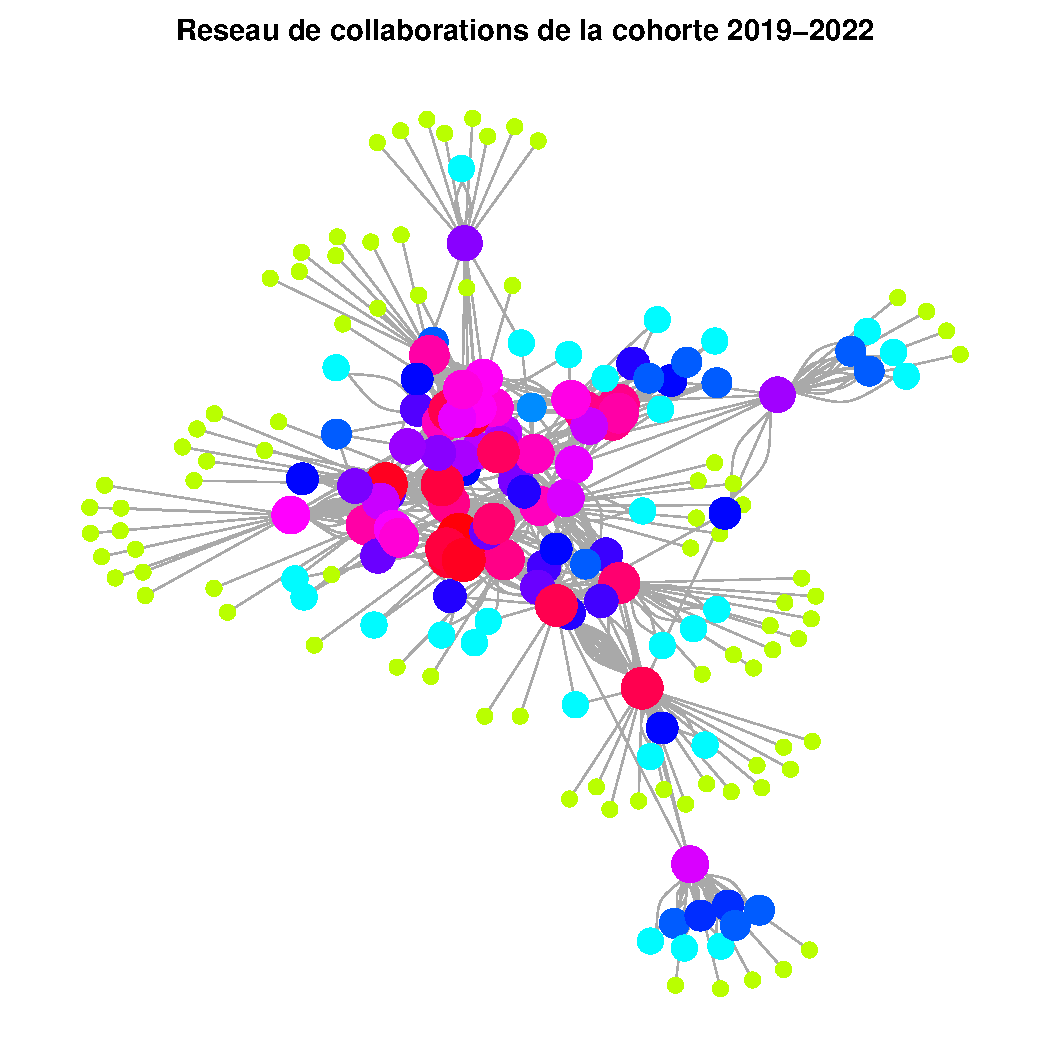
\includegraphics[width=0.5\textwidth,height=0.4\textheight]{../results/reseau.pdf}
\caption{Réseau de collaboration \label{fig:plot1}}
\end{figure}

La figure \ref{fig:plot1} montre le réseau de collaborations, soit la
position des étudiants en fonction du nombre de liens les un par rapport
aux autres. On observe les points, représentant les étudiants, relié par
leurs collaborations avec les autre points entre eux. Dans cette figure,
on retrouve des points plus gros plus au centre de la figure
représentant les étudants ayant le plus de collaborations et des points
plus petits vers l'extérieur de la figure représentant les étudiant
ayant moins de collaboration.

\begin{figure}
\centering
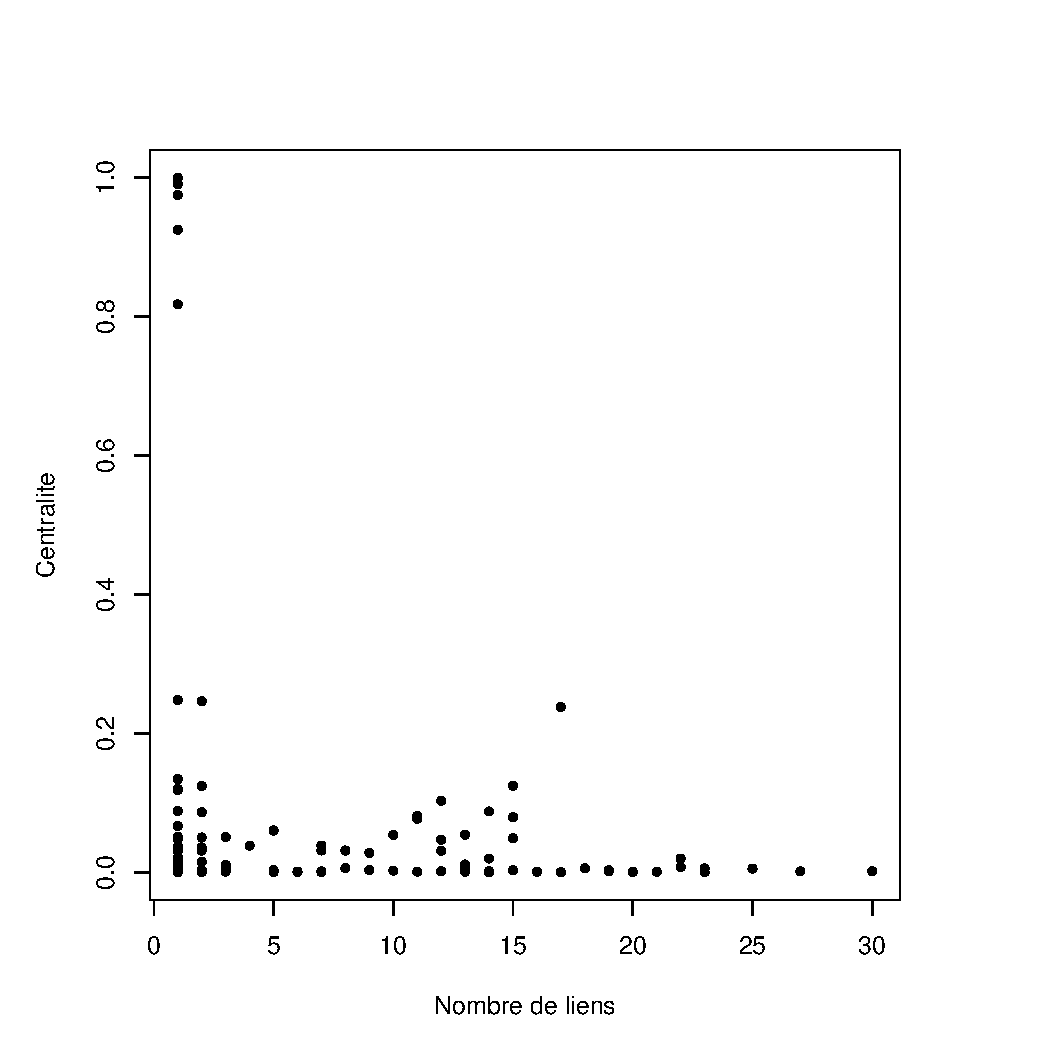
\includegraphics[width=0.5\textwidth,height=0.4\textheight]{../results/centralite.pdf}
\caption{Relation entre la centralité et le nombre de lien
\label{fig:plot2}}
\end{figure}

La figure \ref{fig:plot2} représente la corrélation entre la centralité
et le nombre de lien entre les étudiants. La corrélation effectuée pour
voir le lien entre ces deux facteurs n'est pas significative, car la
corrélation linéaire obtient une valeur de P de 0,2493
(P\textgreater0.05).

\begin{figure}
\centering
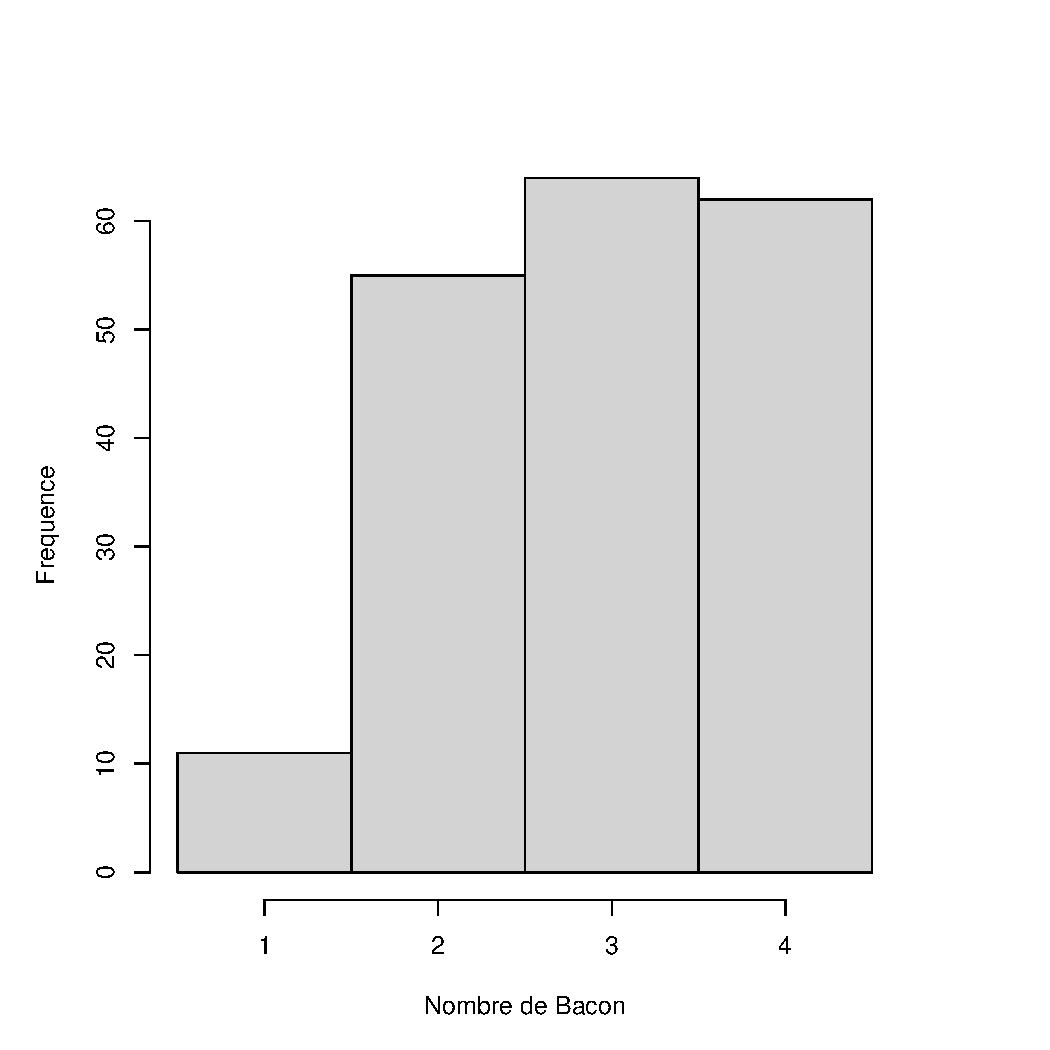
\includegraphics[width=0.5\textwidth,height=0.4\textheight]{../results/bacon.pdf}
\caption{Degré de séparation d'Élisabeth Roy \label{fig:plot3}}
\end{figure}

La figure \ref{fig:plot3} représente le degré de séparation des
étudiants par rapport à l'étudiante Élisabeth Roy. On peut voir que la
majorité des étudiants ont une distance collaborative entre 2 et 4
degrés de séparation avec Élisabeth Roy.

\hypertarget{discussion}{%
\section{Discussion}\label{discussion}}

Le réseau que nous avons obtenu à la Figure \ref{fig:plot1} peut être
considéré comme un réseau de petit monde pour plusieurs raisons. Ce type
de réseau, dont l'exemple parfait est les réseaux sociaux, repose
principalement sur deux caractéristiques. D'abord, la distance moyenne
entre toutes les paires de nœuds d'un réseau de petit monde est faible
(1). Cela est un aspect présent chez les réseaux aléatoires, réseaux
générés par un processus aléatoire. Plus précisément, le degré de
séparation moyens entre les individus doit être aux alentours de six
(1). Cette constatation, démontrée par le sociologue Stanley Milgram,
semble concorder avec notre réseau, dans lequel on peut voir que les
étudiants sont tous à quelques liens seulement des autres étudiants.
Pour un peu de perspective, Facebook a, en 2011, rectifié le nombre de
liens entre ses 2 milliards d'utilisateurs : cette distance médiane est
passé de six à seulement quatre @10.1145/2380718.2380723. Ensuite, pour
qu'un réseau soit considéré comme un petit monde, il faut qu'il
contienne un niveau de regroupement (clustering) local élevé, ce qui
signifie que les nœuds sont généralement très connectés à leurs voisins
immédiats (1). Cette caractéristique n'est pas du tout présente chez les
réseaux aléatoires. On peut également observer cette caractéristique sur
notre réseau, principalement au centre, où l'on trouve des points plus
larges, signifiant qu'ils sont davantage connectés à leurs voisins. Ces
deux propriétés caractérisant les réseaux de petits mondes sont
davantage détaillées dans les prochaines sections.

La Figure \ref{fig:plot2} indique le nombre de lien par des étudiants
rapport à leur centralité dans un réseau de type petit monde. Comme les
réseaux de petits monde sont des réseaux où chacun des noeuds sont
reliés les un avec les autres avec, dans certains cas, des noeuds
intermédiaires pour permettre cette connection (2). Le degrée de
centralité est le nombre de liens relier à un noeud qui peut être
traduit comme étant une mesure d'influence direct d'un noeud (3). Ainsi,
les noeuds intermédiaires ayant plus de liens sont les plus influants.
Cependant, dans notre réseau, cette corrélation n'est pas significative.
Il y a une centralité plus forte chez les étudiant ayant une faible
quantité de lien. Ainsi, la corrélation entre la centralité et le nombre
de lien n'est pas la même que celle retrouvé dans un réseau de type
petit monde. Par contre, plusieurs relations existe par rapport à la
mesure de centralité. Faire l'étude de ses différent rapports pourrait
aider à comprendre la centralité obtenu dans notre figure.

La Figure \ref{fig:plot3} nous indique le nombre de nœuds séparant
Élisabeth Roy des autres étudiant(e)s. Ce nombre varie entre 1 et 4, la
majorité des étudiants ayant un degré de séparation entre 2 et 4 avec
Élisabeth Roy. Cette mesure se réfère directement au Bacon number ou au
Erdös number, basés tout deux sur le phénomène de petit monde. Ces deux
valeurs correspondent à la distance collaborative, d'un côté entre Kevin
Bacon et d'autres acteurs/actrices ayant collaboré dans des films, et de
l'autre entre le mathématicien Paul Erdos et d'autres auteurs/autrices
ayant participé à l'écriture d'articles académiques (4). Selon le
phénomène de petit monde, chaque personne aurait un degré de séparation
avec une autre personne de six maximum, c'est-à-dire que deux personnes
seraient liées par l'entremise de six personnes maximum. Cela concorde
donc avec le résultat que nous avons obtenu à la Figure \ref{fig:plot3},
soit qu'il y a 4 personnes au maximum séparant Élisabeth Roy des autres
étudiant(e)s. Toutefois, cette valeur ne prend en compte qu'une seule
étudiante. Il serait donc intéressant de faire la moyenne de ce même
calcul pour tous les étudiants afin de voir le degré de séparation moyen
entre les individus de notre réseau.

\hypertarget{conclusion}{%
\section{Conclusion}\label{conclusion}}

Le but de ce travail était d'établir si le réseau de collaboration des
étudiants du cours de BIO500 de l'Université de Sherbrooke à l'hiver
2022 concordait avec les caractéristiques d'un réseau de petit monde.
Pour ce faire, une figure représentant le réseau de collaboration des
étudiant entre eux fut produite. Cette figure démontrait une certaine
centralité au niveau des étudiants ayant un nombre de lien plus fort par
rapport à ceux ayant un nombre de lien plus faible. La corrélation entre
le nombre de liens par étudiant et leur centralité dans une figure
n'étant, cependant, pas significative. Par contre, le degré de
séparation, calculé sur un étudiant pris au hazard, correspond au nombre
de degré normalement retrouvé dans un réseau de petit monde. Il n'est
donc pas possible de dire que le réseau de collaboration des étudiants
du cours de BIO500 concorde avec toutes les caractéristiques d'un réseau
de petit monde. Cepandant, des analyses plus poussés pourraient
permettre de mieux comparer ces types de réseau.

\newpage

\hypertarget{bibliographie}{%
\section*{Bibliographie}\label{bibliographie}}
\addcontentsline{toc}{section}{Bibliographie}

\hypertarget{refs}{}
\begin{CSLReferences}{0}{0}
\leavevmode\vadjust pre{\hypertarget{ref-watts_collective_1998}{}}%
\CSLLeftMargin{1. }
\CSLRightInline{Watts DJ, Strogatz SH (1998)
\href{https://doi.org/10.1038/30918}{Collective dynamics of
{``small-world''} networks}. \emph{Nature} 393(6684):440--442.}

\leavevmode\vadjust pre{\hypertarget{ref-uzzi2007small}{}}%
\CSLLeftMargin{2. }
\CSLRightInline{Uzzi B, Amaral LA, Reed-Tsochas F (2007) Small-world
networks and management science research: A review. \emph{European
Management Review} 4(2):77--91.}

\leavevmode\vadjust pre{\hypertarget{ref-borgatti2005centrality}{}}%
\CSLLeftMargin{3. }
\CSLRightInline{Borgatti SP (2005) Centrality and network flow.
\emph{Social networks} 27(1):55--71.}

\leavevmode\vadjust pre{\hypertarget{ref-collins1998s}{}}%
\CSLLeftMargin{4. }
\CSLRightInline{Collins JJ, Chow CC (1998) It's a small world.
\emph{Nature} 393(6684):409--410.}

\end{CSLReferences}



% Bibliography
% \bibliography{pnas-sample}

\end{document}
